\documentclass[a4paper, 10pt]{article}
\usepackage{../CEDT-Homework-style}

\usepackage{amsmath}
\allowdisplaybreaks

\setlength{\headheight}{14.49998pt}

\begin{document}
\subject[2110205 - Statistics for Computer Engineering]
\hwtitle{5}{}{Week 6}{6733172621 Patthadon Phengpinij}{ChatGPT (for\,\LaTeX\,styling and grammar checking)}


% ================================================================================ %
\section{Week 6: Continuous Random Variables}
% ================================================================================ %



% ================================================================================ %
%                                    Problem 01                                    %
% ================================================================================ %
\begin{problem}
For each statement below, determine if it is True or False.
\begin{subproblems}
    \item The value of a Probability Density Function (PDF), \( f(x) \), can be greater than 1.
    \item The value of a Cumulative Distribution Function (CDF), \( F(x) \), can be greater than 1.
    \item The integral of a valid PDF, \( \int_{-\infty}^{\infty} f(x)\,dx \), over its entire range must equal 1.
    \item For any continuous random variable \( X \), the probability \( P(X = c) \) is always 0.
\end{subproblems}
\end{problem}

\begin{solution}
\begin{subproblems}
    \item \boxed{\textbf{True.}} A PDF can take values greater than 1, as long as the total area under the curve equals 1.
    \item \boxed{\textbf{False.}} A CDF must always be between 0 and 1, inclusive.
    \item \boxed{\textbf{True.}} The integral of a valid PDF over its entire range must equal 1, representing the total probability.
    \item \boxed{\textbf{True.}} For continuous random variables, the probability of taking any specific value is 0, since there are infinitely many possible values.
\end{subproblems}
\end{solution}
% ================================================================================ %



% ================================================================================ %
%                                    Problem 02                                    %
% ================================================================================ %
\begin{problem}
A continuous random variable \( X \) has the following piecewise PDF:
\[
f(x) = \begin{cases}
cx & 0 \leq x \le 2 \\
c\paren{4 - x} & 2 \leq x \leq 4 \\
0 & \text{otherwise}
\end{cases}
\]
\begin{subproblems}
    \item Find the value of c that makes \( f(x) \) a valid PDF.
    \item Sketch the graph of the PDF.
\end{subproblems}
\end{problem}

\begin{solution}
For a valid PDF, the total area under the curve must equal 1. We can find \( c \) by integrating \( f(x) \) over its entire range and setting the integral equal to 1.
\begin{align*}
    1 = \int_{-\infty}^{\infty} f(x)\,dx &= \int_{0}^{2} cx\,dx + \int_{2}^{4} c(4 - x)\,dx \\
    &= c \sqbracket{\frac{x^2}{2}}_{0}^{2} + c \sqbracket{4x - \frac{x^2}{2}}_{2}^{4} \\
    &= c \sqbracket{\frac{2^2}{2} - 0 + \paren{4(4) - \frac{4^2}{2}} - \paren{4(2) - \frac{2^2}{2}}} \\
    &= c \sqbracket{2 + (16 - 8) - (8 - 2)} \\
    1 &= c \sqbracket{2 + 8 - 6} = 4c \\
\end{align*}
Thus, the value of \( c \) that would make this PDF valid is: \( \boxed{c = \frac{1}{4}} \; \textbf{a).} \)

This PDF would be:
\[
f(x) = \begin{cases}
    \tfrac{1}{4}x & 0 \leq x \le 2 \\
    \tfrac{1}{4}(4 - x) & 2 \leq x \leq 4 \\
    0 & otherwise
\end{cases}
\]

\textbf{b).} The graph of the PDF is as follows:
\begin{center}
    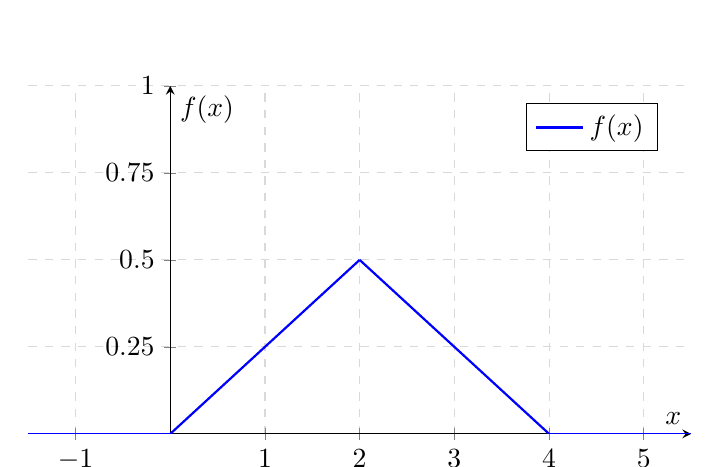
\begin{tikzpicture}
        \begin{axis}[
            axis lines = middle,
            xlabel = \(x\),
            ylabel = {\(f(x)\)},
            ymin = 0, ymax = 1,
            xmin = -1.5, xmax = 5.5,
            xtick = {-1, 0, 1, 2, 3, 4, 5},
            ytick = {0, 0.25, 0.5, 0.75, 1},
            grid = major,
            grid style = {dashed, gray!30},
            width = 10cm, height = 6cm,
            domain = 0:4,
            samples = 100,
            legend style = {at={(0.95,0.95)}, anchor=north east},
            legend cell align = left
        ]
            \addplot[blue, thick, domain=-1.5:0] {0};
            \addplot[blue, thick, domain=0:2] {0.25*x};
            \addplot[blue, thick, domain=2:4] {0.25*(4 - x)};
            \addplot[blue, thick, domain=4:5.5] {0};
            \addlegendentry{\( f(x) \)}
        \end{axis}
    \end{tikzpicture}
\end{center}
\end{solution}
% ================================================================================ %


% ================================================================================ %
%                                    Problem 03                                    %
% ================================================================================ %
\begin{problem}
Using the PDF from Problem 2:
\begin{subproblems}
    \item Calculate the probability \( P(X > 2.5) \).
    \item Derive the Cumulative Distribution Function (CDF), \( F(x) \).
\end{subproblems}
\end{problem}

\begin{solution}
From the previous problem, we have the PDF:
\[
f(x) = \begin{cases}
    \tfrac{1}{4}x & 0 \leq x \le 2 \\
    \tfrac{1}{4}(4 - x) & 2 \leq x \leq 4 \\
    0 & otherwise
\end{cases}
\]

To calculate \( P(X > 2.5) \), we integrate the PDF from 2.5 to 4:
\begin{align*}
    P(X > 2.5) &= \int_{2.5}^{\infty} f(x)\,dx \\
    &= \int_{2.5}^{4} f(x)\,dx + \int_{4}^{\infty} f(x)\,dx \\
    &= \int_{2.5}^{4} \frac{1}{4}(4 - x)\,dx + \int_{4}^{\infty} 0\,dx \\
    &= \frac{1}{4} \sqbracket{4x - \frac{x^2}{2}}_{2.5}^{4} + 0 \\
    &= \frac{1}{4} \sqbracket{(16 - 8) - (10 - 3.125)} \\
    &= \frac{1}{4} \sqbracket{8 - 6.875} \\
    P(X > 2.5) &= \frac{1}{4} \cdot 1.125 = 0.28125
\end{align*}
Thus, \( P(X > 2.5) = \boxed{0.28125} \; \textbf{a).} \)

\vspace{4mm}

To derive the CDF, \( F(x) \), we integrate the PDF from the lower limit to \( x \). \\
Considering the piecewise nature of the PDF, we have:
\begin{align*}
    f(x) &= \begin{cases}
        0 & x \le 0 \\
        \frac{1}{4}x & 0 \leq x \le 2 \\
        \frac{1}{4}(4 - x) & 2 \leq x \le 4 \\
        0 & x \geq 4
    \end{cases} \\ \
    F(x) &= \begin{cases}
        0 & x \le 0 \\
        \int_{0}^{x} \frac{1}{4}t\,dt & 0 \leq x \le 2 \\
        \int_{0}^{2} \frac{1}{4}t\,dt + \int_{2}^{x} \frac{1}{4}(4 - t)\,dt & 2 \leq x \le 4 \\
        1 & x \geq 4
    \end{cases} \\
\end{align*}
Calculating the integrals:
\begin{align*}
    \int_{0}^{x} \frac{1}{4}t\,dt &= \frac{1}{4} \cdot \int_{0}^{x} t\,dt \\
    &= \frac{1}{4} \cdot \sqbracket{\frac{t^2}{2}}_{0}^{x} \\
    &= \frac{1}{4} \cdot \frac{x^2}{2} \\
    \int_{0}^{x} \frac{1}{4}t\,dt &= \frac{x^2}{8} \\
\end{align*}

And:
\begin{align*}
    \int_{2}^{x} \frac{1}{4}(4 - t)\,dt &= \frac{1}{4} \cdot \sqbracket{4t - \frac{t^2}{2}}_{2}^{x} \\
    &= \frac{1}{4} \cdot \paren{(4x - \frac{x^2}{2}) - (8 - 2)} \\
    &= \frac{1}{4} \cdot (4x - \frac{x^2}{2} - 6) \\
    \int_{2}^{x} \frac{1}{4}(4 - t)\,dt &= x - \frac{x^2}{8} - \frac{3}{2} \\
\end{align*}

Thus, the CDF \( F(x) \) is:
\[
F(x) = \begin{cases}
    0 & x < 0 \\
    \frac{x^2}{8} & 0 \leq x \le 2 \\
    \paren{\frac{x^2}{8}}_{x=2} + \paren{x - \frac{x^2}{8} - \frac{3}{2}} & 2 \leq x \le 4 \\
    1 & x \geq 4
\end{cases}
\]
Therefore, the CDF is:
\[
\boxed{F(x) = \begin{cases}
    0 & x < 0 \\
    \frac{x^2}{8} & 0 \leq x < 2 \\
    x - \frac{x^2}{8} - \frac{3}{2} & 2 \leq x < 4 \\
    1 & x \geq 4
\end{cases}} \; \textbf{b).}
\]
\end{solution}
% ================================================================================ %


% ================================================================================ %
%                                    Problem 04                                    %
% ================================================================================ %
\begin{problem}
Using the CDF from Problem 3, find the median of the random variable \( X \).
\end{problem}

\begin{solution}
From the previous problem, we have the CDF:
\[
F(x) = \begin{cases}
    0 & x \leq 0 \\
    \frac{x^2}{8} & 0 \leq x \leq 2 \\
    x - \frac{3}{2} & 2 \leq x \leq 4 \\
    1 & x \geq 4
\end{cases}
\]

For a random variable \( X \), the median is the value \( m \) such that \( F(m) = 0.5 \).
To find the median, we need to solve for \( m \) in the equation \( F(m) = 0.5 \).
We consider the piecewise nature of the CDF:
\begin{enumerate}
    \item For \( 0 \leq m \leq 2 \):
    \[
    F(m) = \frac{m^2}{8} = 0.5
    \]
    Solving for \( m \):
    \[
    m^2 = 4 \implies m = 2 \implies m \in [0, 2], \underline{\textbf{valid.}}
    \]
    
    \item For \( 2 \leq m \leq 4 \):
    \[
    F(m) = m - \frac{3}{2} = 0.5
    \]
    Solving for \( m \):
    \[
    m = 2 \implies m \in [2, 4], \underline{\textbf{valid.}}
    \]
\end{enumerate}

Thus, the median of the random variable \( X \) is \( \boxed{2} \).
\end{solution}
% ================================================================================ %


% ================================================================================ %
%                                    Problem 05                                    %
% ================================================================================ %
\begin{problem}
A shuttle bus arrives at a student dormitory at a random time within a 15-minute window, from 8:00 AM to 8:15 AM.
Let \( T \) be the student's waiting time in minutes if they arrive at exactly 8:00 AM.
\begin{subproblems}
    \item What is the distribution of \( T \)? (Specify type and parameters).
    \item What is the probability that a student waits for more than 10 minutes?
\end{subproblems}
\end{problem}

\begin{solution}
\textbf{a).} The waiting time \( T \) follows a uniform distribution over the interval [0, 15] minutes.
Thus, we can denote this as: \( T \sim \text{Uniform}(0, 15) \)

\vspace{3mm}

\textbf{b).} To find the probability that a student waits for more than 10 minutes: \( P(T > 10) \).
The PDF of a uniform distribution over the interval [a, b] is given by:
\[
f_T(t) = \begin{cases}
    \frac{1}{b-a} & a \leq t \leq b \\
    0 & \text{otherwise}
\end{cases}
\]
For our case, \( a = 0 \) and \( b = 15 \), so the PDF is:
\[
f_T(t) = \begin{cases}
    \frac{1}{15} & 0 \leq t \leq 15 \\
    0 & \text{otherwise}
\end{cases}
\]
To find \( P(T > 10) \), we can integrate the PDF from 10 to 15:
\[
P(T > 10) = \int_{10}^{15} f_T(t) \, dt = \int_{10}^{15} \frac{1}{15} \, dt = \frac{1}{15} \cdot (15 - 10) = \frac{5}{15} = \frac{1}{3}
\]
Thus, the probability that a student waits for more than 10 minutes is \( \boxed{\frac{1}{3}} \).
\end{solution}
% ================================================================================ %


% ================================================================================ %
%                                    Problem 06                                    %
% ================================================================================ %
\begin{problem}
For the shuttle bus scenario in Problem 5:
\begin{subproblems}
    \item What is the expected waiting time, \( \text{E}[T] \)?
    \item What is the variance of the waiting time, \( \text{Var}(T) \)?
\end{subproblems}
\end{problem}

\begin{solution}
From Problem 5, we know that \( T \sim \text{Uniform}(0, 15) \).

\vspace{3mm}

For a uniform distribution \( \text{Uniform}(a, b) \):
\begin{itemize}
    \item The expected value \( \text{E}[X] = \frac{a + b}{2} \)
    \item The variance \( \text{Var}(X) = \frac{(b - a)^2}{12} \)
\end{itemize}

The expected waiting time \( \text{E}[T] \) is:
\[ \text{E}[T] = \frac{0 + 15}{2} = \frac{15}{2} = \boxed{7.5 \text{ minutes}} \; \textbf{a).} \]
The variance of the waiting time \( \text{Var}(T) \) is:
\[ \text{Var}(T) = \frac{(15 - 0)^2}{12} = \frac{225}{12} = \boxed{18.75 \text{ minutes}^2}  \; \textbf{b).} \]
\end{solution}
% ================================================================================ %


% ================================================================================ %
%                                    Problem 07                                    %
% ================================================================================ %
\begin{tosubmit}
\problem
For the shuttle bus scenario in Problem 5, what is the \( 80^\text{th} \) percentile of the waiting time?
In other words, find the time \( t \) (in minutes) such that 80\% of waiting times are less than \( t \).

\vspace{3mm}

\par\noindent\submitsolution
From Problem 5, we know that \( T \sim \text{Uniform}(0, 15) \). \newline
The CDF of a uniform distribution \( \text{Uniform}(a, b) \) is given by:
\[
F_T(t) = \begin{cases}
    0 & t < a \\
    \frac{t - a}{b - a} & a \leq t \leq b \\
    1 & t > b
\end{cases}
\]
For our case, \( a = 0 \) and \( b = 15 \), so the CDF is:
\[
F_T(t) = \begin{cases}
    0 & t < 0 \\
    \frac{t}{15} & 0 \leq t \leq 15 \\
    1 & t > 15
\end{cases}
\]
To find the 80th percentile, we need to solve for \( t \) in the equation \( F_T(t) = 0.8 \):
\[\frac{t}{15} = 0.8 \]
Solving for \( t \):
\[ t = 0.8 \times 15 = 12 \]
Thus, the 80th percentile of the waiting time is \( \boxed{12 \text{ minutes}} \).
\end{tosubmit}
% ================================================================================ %


\end{document}